%%%%%%%%%%%%%%%%%%%%%%%%%%%%%%%%%%%%%%%%%%%%%%%%%%%%%%%%%%%%%%%%%%%%%%%%%%%%%%%%
\documentclass[twocolumn]{revtex4}

%%%%%%%%%%%%%%%%%%%%%%%%%%%%%%%%%%%%%%%%%%%%%%%%%%%%%%%%%%%%%%%%%%%%%%%%%%%%%%%%
% Note that comments begin with a "%" and are not turned into text in the .pdf
% document.
%%%%%%%%%%%%%%%%%%%%%%%%%%%%%%%%%%%%%%%%%%%%%%%%%%%%%%%%%%%%%%%%%%%%%%%%%%%%%%%%

%%%%%%%%%%%%%%%%%%%%%%%%%%%%%%%%%%%%%%%%%%%%%%%%%%%%%%%%%%%%%%%%%%%%%%%%%%%%%%%%
% Include some extra packages.
%%%%%%%%%%%%%%%%%%%%%%%%%%%%%%%%%%%%%%%%%%%%%%%%%%%%%%%%%%%%%%%%%%%%%%%%%%%%%%%%
\usepackage[]{graphicx}
%%%%%%%%%%%%%%%%%%%%%%%%%%%%%%%%%%%%%%%%%%%%%%%%%%%%%%%%%%%%%%%%%%%%%%%%%%%%%%%%

%%%%%%%%%%%%%%%%%%%%%%%%%%%%%%%%%%%%%%%%%%%%%%%%%%%%%%%%%%%%%%%%%%%%%%%%%%%%%%%%
\begin{document}
Dominic Pellino

%%%%%%%%%%%%%%%%%%%%%%%%%%%%%%%%%%%%%%%%%%%%%%%%%%%%%%%%%%%%%%%%%%%%%%%%%%%%%%%%
\title{
Journal article
}

\author{M.~Bellis}
\author{R.~Feynman}
\affiliation{Siena College, Loudonville, NY}

\date{\today}

\begin{abstract}
 So in this final project for software classs we had to make a plot of two equations. With this plot we got a point at which the raptor caught up to the human. The results I got were 2 seconds and 36 meters. But, we couldn't just take the info from the graph, we had to write a code for it. The code i wrote gave me the correct results. After that we had to figure out how long it took for the raptor to be one meter behind the human and how far the human traveled before that time occurred. I got 1.934 seconds and  Finally at the end of the coding we had to find the probability that the raptor would bite us and we are dead or if the human got away. 
\end{abstract}

\maketitle
%%%%%%%%%%%%%%%%%%%%%%%%%%%%%%%%%%%%%%%%%%%%%%%%%%%%%%%%%%%%%%%%%%%%%%%%%%%%%%%%

%%%%%%%%%%%%%%%%%%%%%%%%%%%%%%%%%%%%%%%%%%%%%%%%%%%%%%%%%%%%%%%%%%%%%%%%%%%%%%%%
\section{Introduction}
This project was very difficult for me but through alot of hard work and help from my friends and teacher I was able to get through it. We had four question. Once I was able to figure everything out and it clicked it kind of became fun. So in the future I would like to do more computer programming.

\subsection{Question 1}
In question one we had to create a graph of the position versus time for both the human and the 'raptor plotted on the same graph. We had to clearly label all axes and give the plot a legend. Also we had to plot over a suitable time frame and save the figure as a .png file. I created the plot by plotting both equations one as xhuman and one a xraptor. In this graph there was an intersection between the graphs. this was the point I am looking for in part 2. I 

\subsection{Question 2}
In question 2 we had to figure out how long it took the velociraptor to catch up to the human and how far the human traveled before that occurrence. We could not just look at the graph from problem one and give that as our answer. We had to write another code which gave us the answer. This was confusing for me at first but, i got through it and got the answer. I had to use a while loop to loop over the data points until it gave me the point where the two lines met. That was at 2 seconds and 36 meters. 

\subsection{Question 3}
In question 3 I did basically the same exact thing from part 2 but, this time I had to determine the distance and time when the raptor is one meter behind the human. I had to use a while loop to loop over the data points until it gave me the point where the two lines met. That was at 1.934 seconds and 35.802 meters. Once I got part 2 it was very easy to do part 3. 
%%%%%%%%%%%%%%%%%%%%%%%%%%%%%%%%%%%%%%%%%%%%%%%%%%%%%%%%%%%%%%%%%%%%%%%%%%%%%%%%


%%%%%%%%%%%%%%%%%%%%%%%%%%%%%%%%%%%%%%%%%%%%%%%%%%%%%%%%%%%%%%%%%%%%%%%%%%%%%%%%
\pagebreak
\section{Other stuff}

The equation I used was: 
$$x_f = v_0t + x_0$$
My results for question 2 were 2 seconds and 36 meters.
My results for question 3 were 1.934 seconds and 35.802 meters.
Question 4 I really did not understand. So i was not able to do it. 
%%%%%%%%%%%%%%%%%%%%%%%%%%%%%%%%%%%%%%%%%%%%%%%%%%%%%%%%%%%%%%%%%%%%%%%%%%%%%%%%
\begin{figure}[h]

\begin{center}
	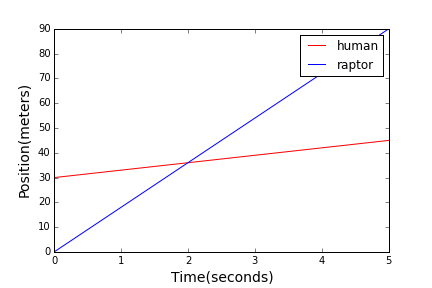
\includegraphics[width=0.5\textwidth]{Human_Raptor_Linegraph.png}
	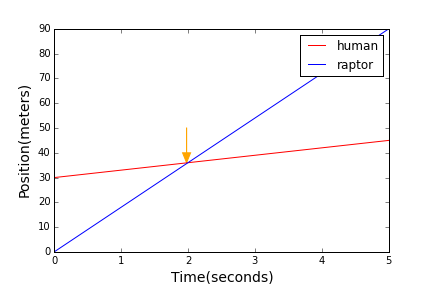
\includegraphics[width=0.5\textwidth]{graph_with_arrow.png}
	
\end{center}

\end{figure}
\pagebreak
%%%%%%%%%%%%%%%%%%%%%%%%%%%%%%%%%%%%%%%%%%%%%%%%%%%%%%%%%%%%%%%%%%%%%%%%%%%%%%%%
\end{document}
%%%%%%%%%%%%%%%%%%%%%%%%%%%%%%%%%%%%%%%%%%%%%%%%%%%%%%%%%%%%%%%%%%%%%%%%%%%%%%%%
